%%%%%%%%%%%%%%%%%%%%%%%%%%%%%%%%%%%%%%%%%%%%%%%%%%%%%%%%%%%%%%%%%%%%
%% I, the copyright holder of this work, release this work into the
%% public domain. This applies worldwide. In some countries this may
%% not be legally possible; if so: I grant anyone the right to use
%% this work for any purpose, without any conditions, unless such
%% conditions are required by law.
%%%%%%%%%%%%%%%%%%%%%%%%%%%%%%%%%%%%%%%%%%%%%%%%%%%%%%%%%%%%%%%%%%%%

\documentclass{beamer}
\usetheme[faculty=phil]{fibeamer}
\usepackage{polyglossia}  %% By using `czech` or `slovak` as the
\setmainlanguage{english} %% main locale instead of `english`, you
%% can typeset the presentation in either Czech or Slovak,
%% respectively.
\setotherlanguages{czech, slovak} %% The additional keys allow
%%
%%   \begin{otherlanguage}{czech}   ... \end{otherlanguage}
%%   \begin{otherlanguage}{slovak}  ... \end{otherlanguage}
%%
%% These macros specify information about the presentation
\title{Presentation Title} %% that will be typeset on the
\subtitle{Presentation Subtitle} %% title page.
\author{Author's Name}
%% These additional packages are used within the document:
\usepackage{ragged2e}  % `\justifying` text
\usepackage{booktabs}  % Tables
\usepackage{tabularx}
\usepackage{tikz}      % Diagrams
\usetikzlibrary{calc, shapes, backgrounds}
\usepackage{amsmath, amssymb}
\usepackage{url}       % `\url`s
\usepackage{listings}  % Code listings
\frenchspacing
\begin{document}
  \frame{\maketitle}

  \AtBeginSection[]{% Print an outline at the beginning of sections
    \begin{frame}<beamer>
      \frametitle{Outline for Section \thesection}
      \tableofcontents[currentsection]
    \end{frame}}

    \section{Light Frames}
    \subsection{Blind Text}
    \begin{frame}{Jabberwocky}
      \framesubtitle{Lewis Carroll}%
      \begin{tikzpicture}[overlay,remember picture]
        \node[anchor=south east,xshift=-30pt,yshift=35pt]
          at (current page.south east) {
            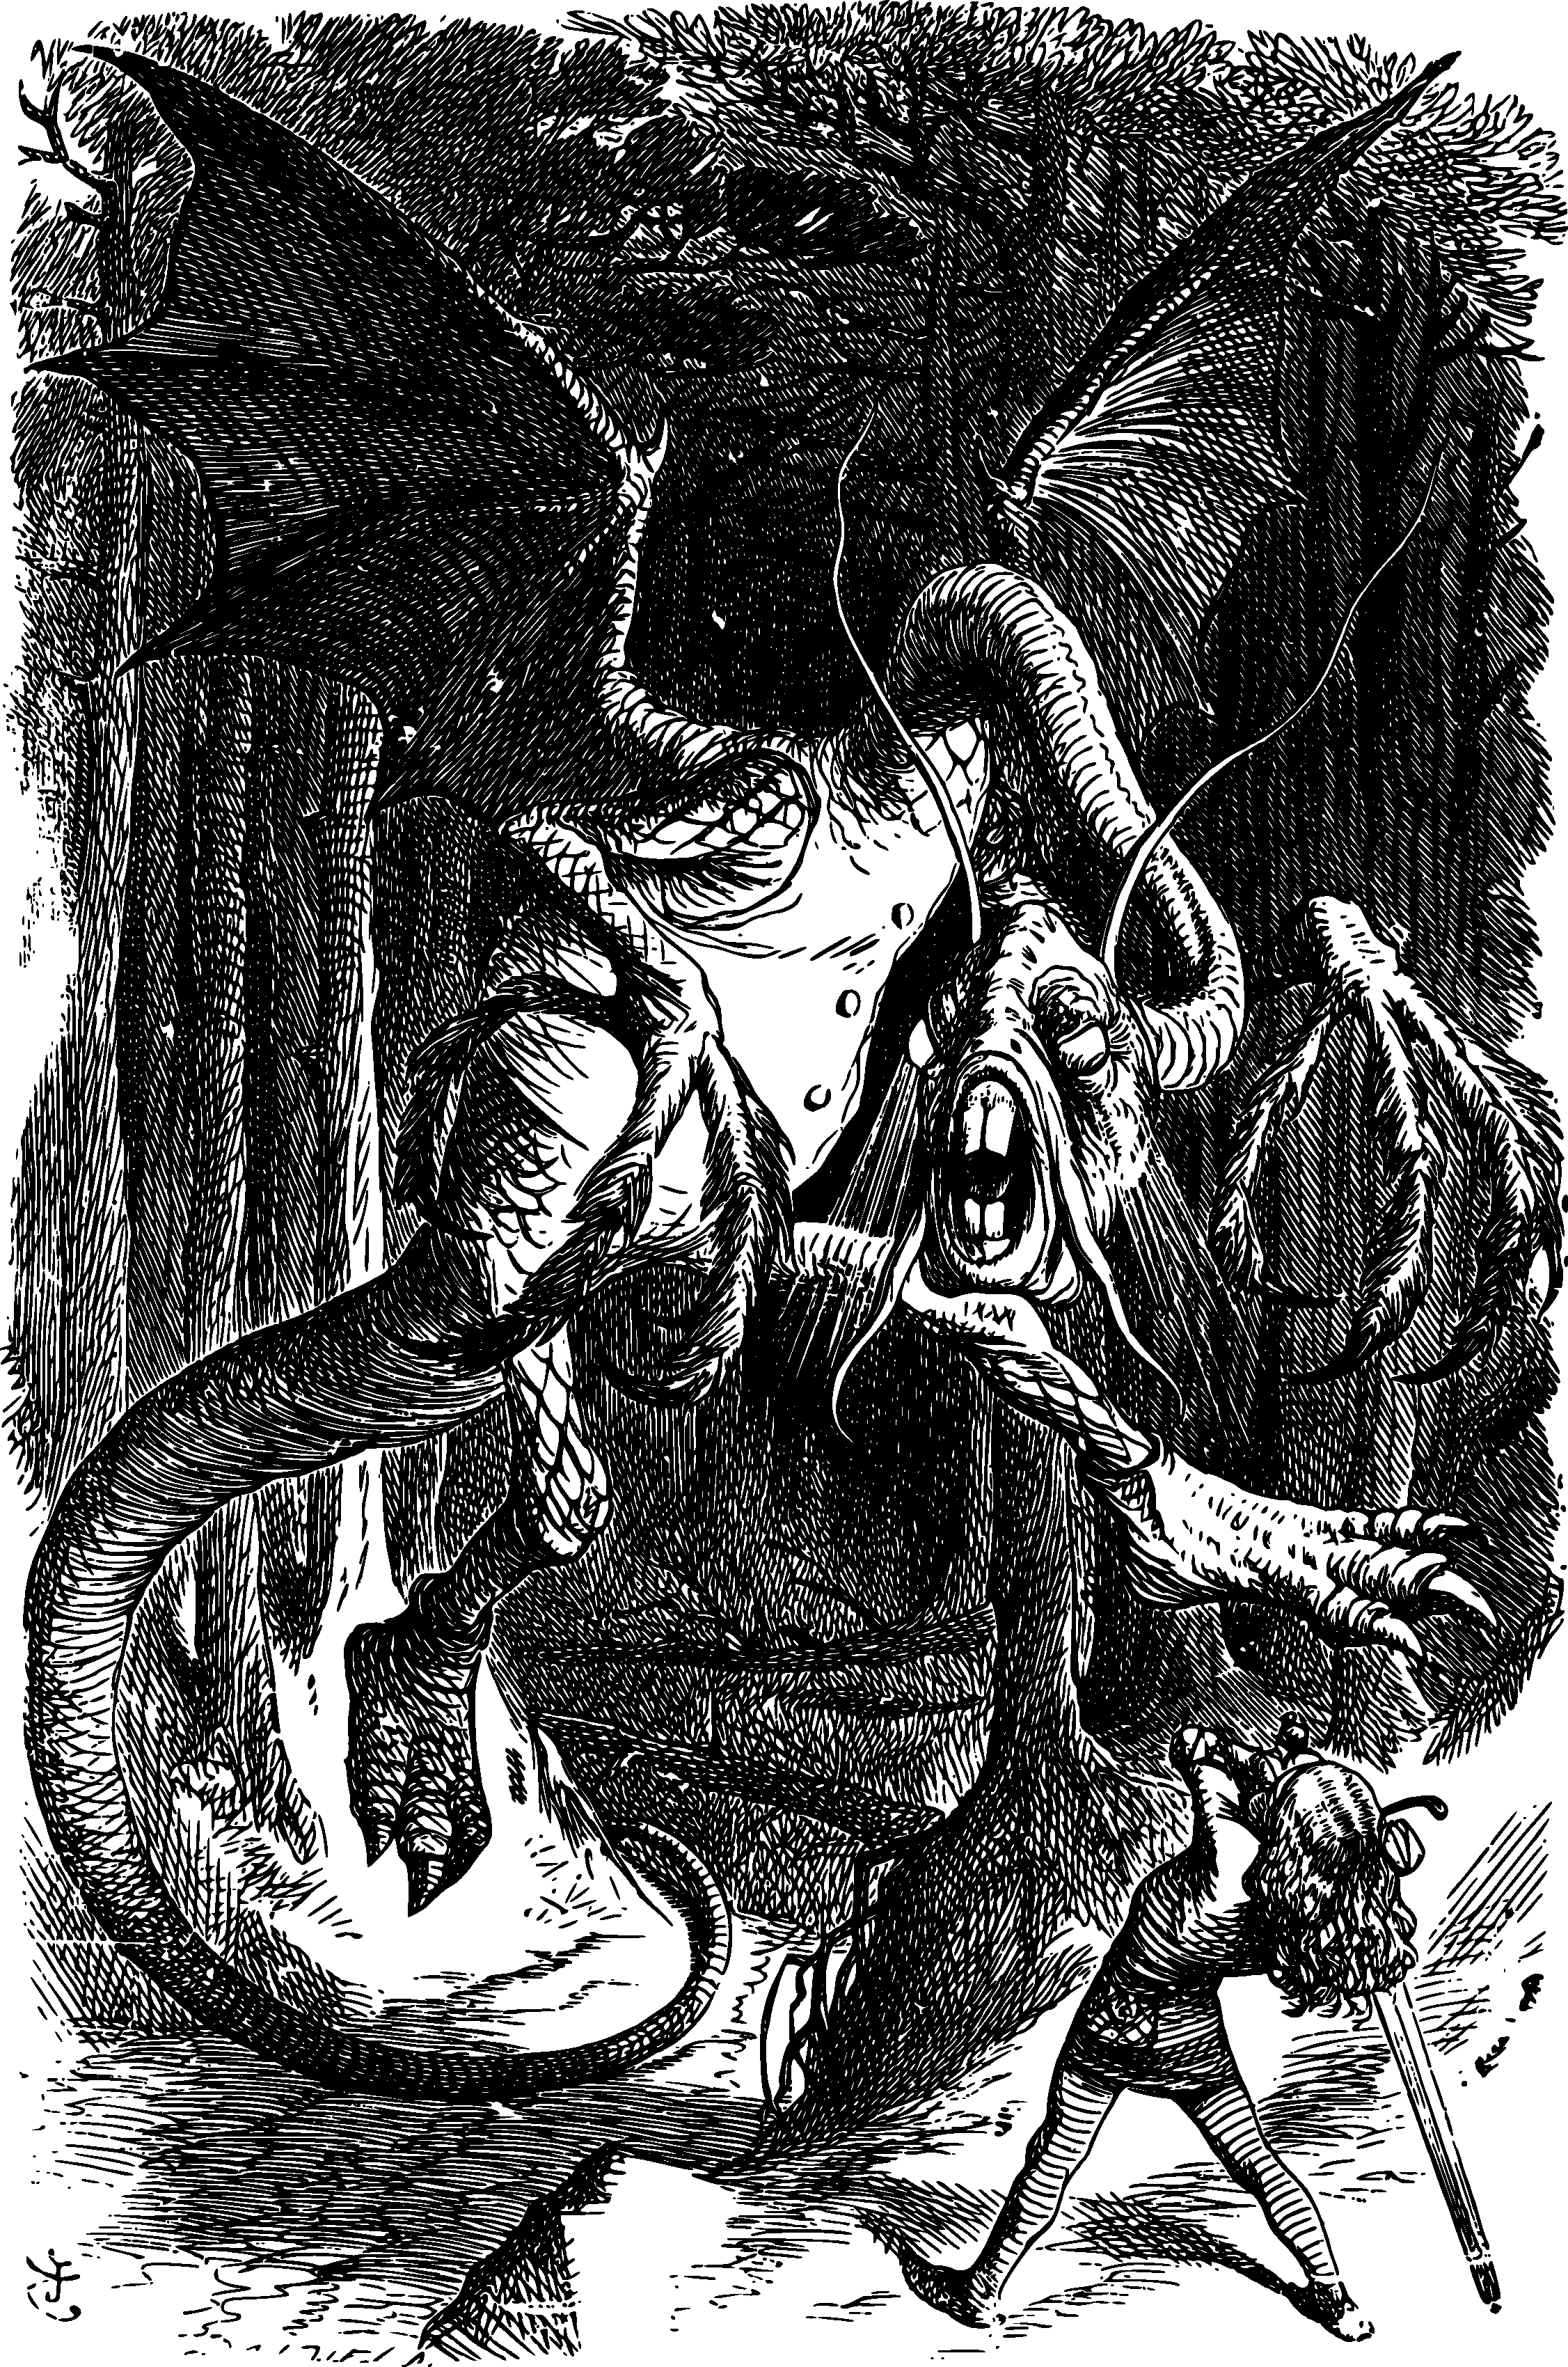
\includegraphics[width=35mm]{resources/jabberwocky-light}
          };
      \end{tikzpicture}%
      'Twas brillig, and the slithy toves\\
      Did gyre and gimble in the wabe;\\
      All mimsy were the borogoves,\\
      And the mome raths outgrabe.\\\bigskip

      “Beware the Jabberwock, my son!\\
      The jaws that bite, the claws that catch!\\
      Beware the Jubjub bird, and shun\\
      The frumious Bandersnatch!”\\
    \end{frame}

    \begin{frame}[label=lists]{Lists and locales}
      \framesubtitle{Lorem ipsum dolor sit amet}
      \begin{columns}[onlytextwidth]
        \column{.5\textwidth}
          \begin{itemize}
            \item Nulla nec lacinia odio. Curabitur urna tellus.
            \begin{itemize}
              \item Fusce id sodales dolor. Sed id metus dui.
              \begin{itemize}
                \item Cupio virtus licet mi vel feugiat.
              \end{itemize}
            \end{itemize}
          \end{itemize}
        \column{.5\textwidth}
          \begin{enumerate}
            \item Donec porta, risus porttitor egestas scelerisque video.
            \begin{enumerate}
              \item Nunc non ante fringilla, manus potentis cario.
              \begin{enumerate}
                \item Pellentesque servus morbi tristique.
              \end{enumerate}
            \end{enumerate}
          \end{enumerate}
      \end{columns}
      \bigskip
      \justifying

      {\uselanguage{czech}Nechť již hříšné saxofony ďáblů
      rozzvučí síň úděsnými tóny waltzu, tanga a quickstepu!}
      {\uselanguage{slovak} Nezvyčajné kŕdle šťastných figliarskych
      ďatľov učia pri kótovanom ústí Váhu mĺkveho koňa Waldemara
      obžierať väč\-šie kusy exkluzívnej kôry.}
      {\uselanguage{english}The quick, brown fox jumps over a lazy
      dog. DJs flock by when MTV ax quiz prog. “Now fax quiz Jack!”}
    \end{frame}

    \subsection{Structuring Elements}
    \begin{frame}[label=simmonshall]{Text blocks}
      \framesubtitle{In plain, example, and \alert{alert} flavour}
      \alert{This text} is highlighted.

      \begin{block}{A plain block}
        This is a plain block containing some \alert{highlighted text}.
      \end{block}
      \begin{exampleblock}{An example block}
        This is an example block containing some \alert{highlighted text}.
      \end{exampleblock}
      \begin{alertblock}{An alert block}
        This is an alert block containing some \alert{highlighted text}.
      \end{alertblock}
    \end{frame}

    \begin{frame}[label=proof]{Definitions, theorems, and proofs}
      \framesubtitle{All integers divide zero}
      \begin{definition}
        $\forall a,b\in\mathds{Z}: a\mid b\iff\exists c\in\mathds{Z}:a\cdot c=b$
      \end{definition}
      \begin{theorem}
        $\forall a\in\mathds{Z}: a\mid 0$
      \end{theorem}
      \begin{proof}[Proof\nopunct]
        $\forall a\in\mathds{Z}: a\cdot 0=0$
      \end{proof}
    \end{frame}

    \subsection{Numerals and Mathematics}
    \begin{frame}[label=math]{Numerals and Mathematics}
      \framesubtitle{Formulae, equations, and expressions}
      \begin{columns}[onlytextwidth]
        \column{.20\textwidth}
          1234567890
        \column{.20\textwidth}
          \oldstylenums{1234567890}
        \column{.20\textwidth}
          $\hat{x}$, $\check{x}$, $\tilde{a}$,
          $\bar{a}$, $\dot{y}$, $\ddot{y}$
        \column{.40\textwidth}
          $\int \!\! \int f(x,y,z)\,\mathsf{d}x\mathsf{d}y\mathsf{d}z$
      \end{columns}
      \begin{columns}[onlytextwidth]
        \column{.5\textwidth}
          $$\frac{1}{\displaystyle 1+
            \frac{1}{\displaystyle 2+
            \frac{1}{\displaystyle 3+x}}} +
            \frac{1}{1+\frac{1}{2+\frac{1}{3+x}}}$$
        \column{.5\textwidth}
          $$F:\left| \begin{array}{ccc}
          F''_{xx} & F''_{xy} &  F'_x \\
          F''_{yx} & F''_{yy} &  F'_y \\
          F'_x     & F'_y     & 0
          \end{array}\right| = 0$$
      \end{columns}
      \begin{columns}[onlytextwidth]
        \column{.3\textwidth}
          $$\mathop{\int \!\!\! \int}_{\mathbf{x} \in \mathds{R}^2}
          \! \langle \mathbf{x},\mathbf{y}\rangle\,\mathsf{d}\mathbf{x}$$
        \column{.33\textwidth}
          $$\overline{\overline{a\alpha}^2+\underline{b\beta}
           +\overline{\overline{d\delta}}}$$
        \column{.37\textwidth}
          $\left] 0,1\right[ + \lceil x \rfloor - \langle x,y\rangle$
      \end{columns}
      \begin{columns}[onlytextwidth]
        \column{.4\textwidth}
          \begin{eqnarray*}
           e^x &\approx& 1+x+x^2/2! + \\
             && {}+x^3/3! + x^4/4!
          \end{eqnarray*}
        \column{.6\textwidth}
          $${n+1\choose k} = {n\choose k} + {n \choose k-1}$$
      \end{columns}
    \end{frame}

    \subsection{Figures and Code Listings}
    \begin{frame}[label=figs1]{Figures}
      \framesubtitle{Tables, graphs, and images}
      \begin{table}[!b]
        {\carlitoTLF % Use monospaced lining figures
        \begin{tabularx}{\textwidth}{Xrrr}
          \textbf{Faculty} & \textbf{With \TeX} & \textbf{Total} &
          \textbf{\%} \\
          \toprule
          Faculty of Informatics       & 1\,716  & 2\,904  &
          59.09 \\% 1433
          Faculty of Science           & 786     & 5\,275  &
          14.90 \\% 1431
          Faculty of $\genfrac{}{}{0pt}{}{\textsf{Economics and}}{%
          \textsf{Administration}}$    & 64      & 4\,591  &
          1.39  \\% 1456
          Faculty of Arts              & 69      & 10\,000 &
          0.69  \\% 1421
          Faculty of Medicine          & 8       & 2\,014  &
          0.40  \\% 1411
          Faculty of Law               & 15      & 4\,824  &
          0.31  \\% 1422
          Faculty of Education         & 19      & 8\,219  &
          0.23  \\% 1441
          Faculty of Social Studies    & 12      & 5\,599  &
          0.21  \\% 1423
          Faculty of Sports Studies    & 3       & 2\,062  &
          0.15  \\% 1451
          \bottomrule
        \end{tabularx}}
        \caption{The distribution of theses written using \TeX\ during 2010--15 at MU}
      \end{table}
    \end{frame}
    \begin{frame}[label=figs2]{Figures}
      \framesubtitle{Tables, graphs, and images}
      \begin{figure}[b]
        \centering
        % Flipping a coin
        % Author: cis
        \tikzset{
          head/.style = {fill = none, label = center:\textsf{H}},
          tail/.style = {fill = none, label = center:\textsf{T}}}
        \scalebox{0.65}{\begin{tikzpicture}[
            scale = 1.5, transform shape, thick,
            every node/.style = {draw, circle, minimum size = 10mm},
            grow = down,  % alignment of characters
            level 1/.style = {sibling distance=3cm},
            level 2/.style = {sibling distance=4cm},
            level 3/.style = {sibling distance=2cm},
            level distance = 1.25cm
          ]
          \node[shape = rectangle,
            minimum width = 6cm, font = \sffamily] {Coin flipping}
          child { node[shape = circle split, draw, line width = 1pt,
                  minimum size = 10mm, inner sep = 0mm, rotate = 30] (Start)
                  { \rotatebox{-30}{H} \nodepart{lower} \rotatebox{-30}{T}}
           child {   node [head] (A) {}
             child { node [head] (B) {}}
             child { node [tail] (C) {}}
           }
           child {   node [tail] (D) {}
             child { node [head] (E) {}}
             child { node [tail] (F) {}}
           }
          };

          % Filling the root (Start)
          \begin{scope}[on background layer, rotate=30]
            \fill[head] (Start.base) ([xshift = 0mm]Start.east) arc (0:180:5mm)
              -- cycle;
            \fill[tail] (Start.base) ([xshift = 0pt]Start.west) arc (180:360:5mm)
              -- cycle;
          \end{scope}

          % Labels
          \begin{scope}[nodes = {draw = none}]
            \path (Start) -- (A) node [near start, left]  {$0.5$};
            \path (A)     -- (B) node [near start, left]  {$0.5$};
            \path (A)     -- (C) node [near start, right] {$0.5$};
            \path (Start) -- (D) node [near start, right] {$0.5$};
            \path (D)     -- (E) node [near start, left]  {$0.5$};
            \path (D)     -- (F) node [near start, right] {$0.5$};
            \begin{scope}[nodes = {below = 11pt}]
              \node [name = X] at (B) {$0.25$};
              \node            at (C) {$0.25$};
              \node [name = Y] at (E) {$0.25$};
              \node            at (F) {$0.25$};
            \end{scope}
          \end{scope}
        \end{tikzpicture}}
        \caption{Tree of probabilities -- Flipping a coin\footnote[frame]{%
          A derivative of a diagram from \url{texample.net} by cis, CC BY 2.5 licensed}}
      \end{figure}
    \end{frame}

    \defverbatim[colored]\sleepSort{
      \begin{lstlisting}[language=C,tabsize=2]
  #include <stdio.h>
  #include <unistd.h>
  #include <sys/types.h>
  #include <sys/wait.h>

  // This is a comment
  int main(int argc, char **argv)
  {
          while (--c > 1 && !fork());
          sleep(c = atoi(v[c]));
          printf("%d\n", c);
          wait(0);
          return 0;
  }
    \end{lstlisting}}
    \begin{frame}{Code listings}{An example source code in C}
      \sleepSort
    \end{frame}

    \subsection{Citations and Bibliography}
    \begin{frame}[label=citations]{Citations}
      \framesubtitle{\TeX, \LaTeX, and Beamer}

      \justifying\TeX\ is a programming language for the typesetting
      of documents. It was created by Donald Erwin Knuth in the late
      1970s and it is documented in \emph{The \TeX
      book}~\cite{knuth84}.

      In the early 1980s, Leslie Lamport created the initial version
      of \LaTeX, a high-level language on top of \TeX, which is
      documented in \emph{\LaTeX : A Document Preparation
      System}~\cite{lamport94}. There exists a healthy ecosystem of
      packages that extend the base functionality of \LaTeX;
      \emph{The \LaTeX\ Companion}~\cite{MG94} acts as a guide
      through the ecosystem.

      In 2003, Till Tantau created the initial version of Beamer, a
      \LaTeX\ package for the creation of presentations. Beamer is
      documented in the \emph{User's Guide to the Beamer
      Class}~\cite{tantau04}.
    \end{frame}

    \begin{frame}[label=bibliography]{Bibliography}
      \framesubtitle{\TeX, \LaTeX, and Beamer}
      \begin{thebibliography}{9}
        \bibitem{knuth84}
            Donald~E.~Knuth.
            \emph{The \TeX book}.
            Addison-Wesley, 1984.
        \bibitem{lamport94}
            Leslie~Lamport.
            \emph{\LaTeX : A Document Preparation System}.
            Addison-Wesley, 1986.
        \bibitem{MG94}
            M.~Goossens, F.~Mittelbach, and A.~Samarin.
            \emph{The \LaTeX\ Companion}.
            Addison-Wesley, 1994.
        \bibitem{tantau04}
            Till~Tantau.
            \emph{User's Guide to the Beamer Class Version 3.01}.
            Available at \url{http://latex-beamer.sourceforge.net}.
        \bibitem{MS05}
            A.~Mertz and W.~Slough.
            Edited by B.~Beeton and K.~Berry.
            \emph{Beamer by example} In TUGboat,
              Vol. 26, No. 1., pp. 68-73.
      \end{thebibliography}
    \end{frame}

  \section{Dark Frames}
  \begin{darkframes}
    \subsection{Blind Text}
    \begin{frame}{Jabberwocky}
      \framesubtitle{Lewis Carroll}%
      \begin{tikzpicture}[overlay,remember picture]
        \node[anchor=south east,xshift=-30pt,yshift=35pt]
          at (current page.south east) {
            
\includegraphics[width=35mm]{resources/jabberwocky-dark}
          };
      \end{tikzpicture}%
      'Twas brillig, and the slithy toves\\
      Did gyre and gimble in the wabe;\\
      All mimsy were the borogoves,\\
      And the mome raths outgrabe.\\\bigskip

      “Beware the Jabberwock, my son!\\
      The jaws that bite, the claws that catch!\\
      Beware the Jubjub bird, and shun\\
      The frumious Bandersnatch!”\\
    \end{frame}
    \againframe{lists}
    \subsection{Structuring Elements}
    \againframe{simmonshall}
    \againframe{proof}
    \subsection{Numerals and Mathematics}
    \againframe{math}
    \subsection{Figures and Code Listings}
    \againframe{figs1}
    \againframe{figs2}
    \defverbatim[colored]\sleepSort{
      \begin{lstlisting}[language=C,tabsize=2]
#include <stdio.h>
#include <unistd.h>
#include <sys/types.h>
#include <sys/wait.h>

// This is a comment
int main(int argc, char **argv)
{
        while (--c > 1 && !fork());
        sleep(c = atoi(v[c]));
        printf("%d\n", c);
        wait(0);
        return 0;
}
    \end{lstlisting}}
  \begin{frame}{Code listings}{An example source code in C}
      \sleepSort
    \end{frame}
    \subsection{Citations and Bibliography}
    \againframe{citations}
    \againframe{bibliography}
  \end{darkframes}
\end{document}
